\documentclass[a4paper,14pt]{article} % формат документа

\usepackage{cmap} % поиск в ПДФ
\usepackage[T2A]{fontenc} % кодировка
\usepackage[utf8]{inputenc} % кодировка исходного текста
\usepackage[english,russian]{babel} % локализация и переносы
\usepackage[left = 2cm, right = 1cm, top = 2cm, bottom = 2 cm]{geometry} % поля
\usepackage{listings}
\usepackage{graphicx} % для вставки рисунков
\graphicspath{{pictures/}}
\DeclareGraphicsExtensions{.pdf,.png,.jpg}
\newcommand{\anonsection}[1]{\section*{#1}\addcontentsline{toc}{section}{#1}}

\lstset{ %
	language=Python,                % Язык программирования 
	numbers=left,                   % С какой стороны нумеровать          
	frame=single,                    % Добавить рамку
}

\begin{document}
	\begin{titlepage}

       		\begin{center}
         		\large
		
        			Государственное образовательное учреждение высшего профессионального образования\\
       			“Московский государственный технический университет имени Н.Э.Баумана”
         		\vspace{3cm}
            
            		\textsc{Дисциплина: Анализ алгоритмов}
           		\vspace{0.5cm}
                
            		\textsc{Лабораторная работа № 1}
           		 \vspace{3cm}
            
           		 \LARGE 
		 
		 	Расстояния Левенштейна и Дамерау-Левенштейна
           		 \vspace{3cm}
            
            		Студент: Сиденко Анастасия Генадьевна \\   
            		Группа: ИУ7-53Б \\
           		\hfill
            
           		Преподаватели: Строганов Юрий Владимирович \\
           		Волкова Лидия Леонидовна
            		\vfill
            		
			\large
            		2019 г.
		\end{center}

	\end{titlepage}
    
	\tableofcontents
	
	\newpage
    
	\anonsection{Введение}
        
        В данной лабораторной работе ставятся следующие задачи:
        \begin{enumerate} 
		\item Изучение алгоритма Левенштейна и его модификации (алгоритма Дамерау-Левенштейна) для нахождения расстояние между строками
		\item Получение практических навыков реализации данных алгоритма с использованием рекурсии и матрицы на одном из языков программирования
		\item Сравнительный анализ матричного и рекурсивного алгоритмов по затрачиваемым ресурсам (зависимость времени от длины строки)
		\item Экспериментальное подтверждение различий во временной эффективности рекурсивной и матричной реализаций выбранного алгоритма определения расстояния между строками на материале замеров процессорного времени выполнения реализации на варьирующихся длинах строк
	\end{enumerate} 
	
	\newpage


        \section{Аналитическая часть}
        \hfill
        
        Рассмотрим понятия расстояния Левенштейна и расстояния Дамерау-Левенштейна, их использование в настоящее время. 
        
        \subsection{Описание задачи}
        \hfill
        
        \textbf{Расстояние Левенштейна}  (редакционное расстояние) — минимальное количество операций вставки одного символа, удаления одного символа и замены одного символа на другой, необходимых для превращения одной строки в другую.
        
        \hfill
        
        Для двух строк $s1, s2$, их длины $m, n$ соответстсвенно, расстояние Левенштейна равно $D(m, n)$, где
        
        $$
        D(i, j) = 
        \left\{
		\begin{array}{lll}
 			0 , & i = 0, j = 0  \\
			i , & i > 0, j = 0  \\
			j , &i = 0, j > 0 & (1)\\
			min
			\left(
				\begin{array}{lll}
					D(i, j - 1) + 1 \\
					D(i - 1, j ) + 1 \\
					D(i - 1 , j - 1) +  
								\left\{
									\begin{array}{lll}
										0, & s1[i] = s2[j] \\
										1, & else \\
									\end{array}
								\right.\\
				\end{array}
			\right) & j > 0, i > 0
 		\end{array}
	\right.
        $$
         
        \hfill
        
        \textbf{Редакторские операции: }
	\begin{enumerate}
	 	\item I -- Вставка -- штраф 1
	 	\item D -- Удаление -- штраф 1
 	 	\item R -- Замена -- штраф 1
	 	\item M -- Совпадение -- штраф 0
	\end{enumerate}
	
	\hfill
	
	\textbf{Расстояние Дамерау-Левенштейна} -- если к списку разрешённых операций добавить транспозицию (два соседних символа меняются местами), получается расстояние Дамерау — Левенштейна. Дамерау показал, что 80\%  ошибок при наборе текста человеком являются транспозициями. Цена ошибки транспозиции равна 1. 
	
	\hfill
	
	Для двух строк $s1, s2$, их длины $m, n$ соответстсвенно, расстояние Левенштейна равно $D(m, n)$, где
        
        $$
        D(i, j) = 
        \left\{
		\begin{array}{lll}
 			0 , & i = 0, j = 0  \\
			i , & i > 0, j = 0  \\
			j , &i = 0, j > 0\\
			min
			\left(
				\begin{array}{lll}
					D(i, j - 1) + 1 \\
					D(i - 1, j ) + 1 \\
					D(i - 1 , j - 1) +  
								\left\{
									\begin{array}{lll}
										0, & s1[i] = s2[j] \\
										1, & else \\
									\end{array}
								\right.\\
					D(i - 2,j - 2) + 1
				\end{array}
			\right) & i, j > 1, s1[i] = s2[j - 1], s1[i - 1] = s2[j]  & (2)\\
			min
			\left(
				\begin{array}{lll}
					D(i, j - 1) + 1 \\
					D(i - 1, j ) + 1 \\
					D(i - 1 , j - 1) +  
								\left\{
									\begin{array}{lll}
										0, & s1[i] = s2[j] \\
										1, & else \\
									\end{array}
								\right.\\
				\end{array}
			\right) &else
 		\end{array}
	\right.
        $$
        \hfill
        
        \textbf{Расстояние Левенштейна и его модификация активно применяются:}
	\begin{enumerate}
		\item для исправления ошибок в слове (в поисковых системах, базах данных, при вводе текста, при автоматическом распознавании отсканированного текста или речи).
		\item для сравнения текстовых файлов утилитой diff и ей подобными. Здесь роль «символов» играют строки, а роль «строк» — файлы.
		\item в биоинформатике для сравнения генов, хромосом и белков.
	\end{enumerate}
	
        \subsection{Пути решения}
        \hfill
        
        Впервые задачу поставил в 1965 году советский математик Владимир Левенштейн при изучении последовательностей 0-1, а впоследствии более общую задачу для произвольного алфавита связали с его именем. 
        
        \hfill
        
        А пару лет назад Фредерик Дамерау доказал, что большинство ошибок при наборе текста — как раз и есть транспозиции. Поэтому именно данная метрика дает наилучшие результаты на практике.
        
        \hfill
        
        Исходный вариант алгоритма имеет временную сложность O(mn) и потребляет O(mn) памяти, где m и n — длины сравниваемых строк. Весь процесс можно представить матрицей. 
        
           \subsection{Выводы} 
           \hfill
           
           Алгоритмы Дамерау и Дамерау-Левенштейна, для нахождения редакторского расстояния, особо актуальны во время развития технологий и биоинформатики. В основе нахождения минимального расстояния лежат редакторские операции - вставка, удаление, замена, совпадение и транспозиция, которая была введена Дамерау. В данной работе требуется изучить и применить данные алгоритмы, а также получить сравнение реализаций по скорости работы. 
	  
	\newpage

	\section{Конструкторская часть}
	\hfill
	
	В данной работе для нахождения расстояния Левенштейна используется матричный алгоритм, для Дамерау-Левенштейна - матричный и рекурсивный. Рассмотрим и изучим данные варианты реализации. 
	\subsection{IDEF0}
	\hfill
	
	На рисунке 1 показана диаграмма нашего алгоритма.  
	\begin{center}
		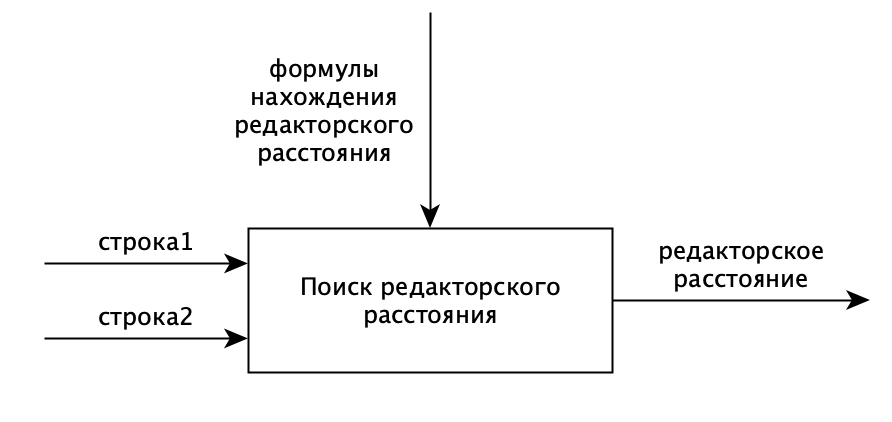
\includegraphics[scale = 0.5]{idef0} \\ Рис.  1 - IDEF0
	\end{center}
        
        \subsection{Схемы алгоритмов}
        Приведем схемы 3 исследуемых нами алгоритмов. 
        
        \subsubsection{Расстояние Левенштейна матричным способом}
        
        \begin{center}
        		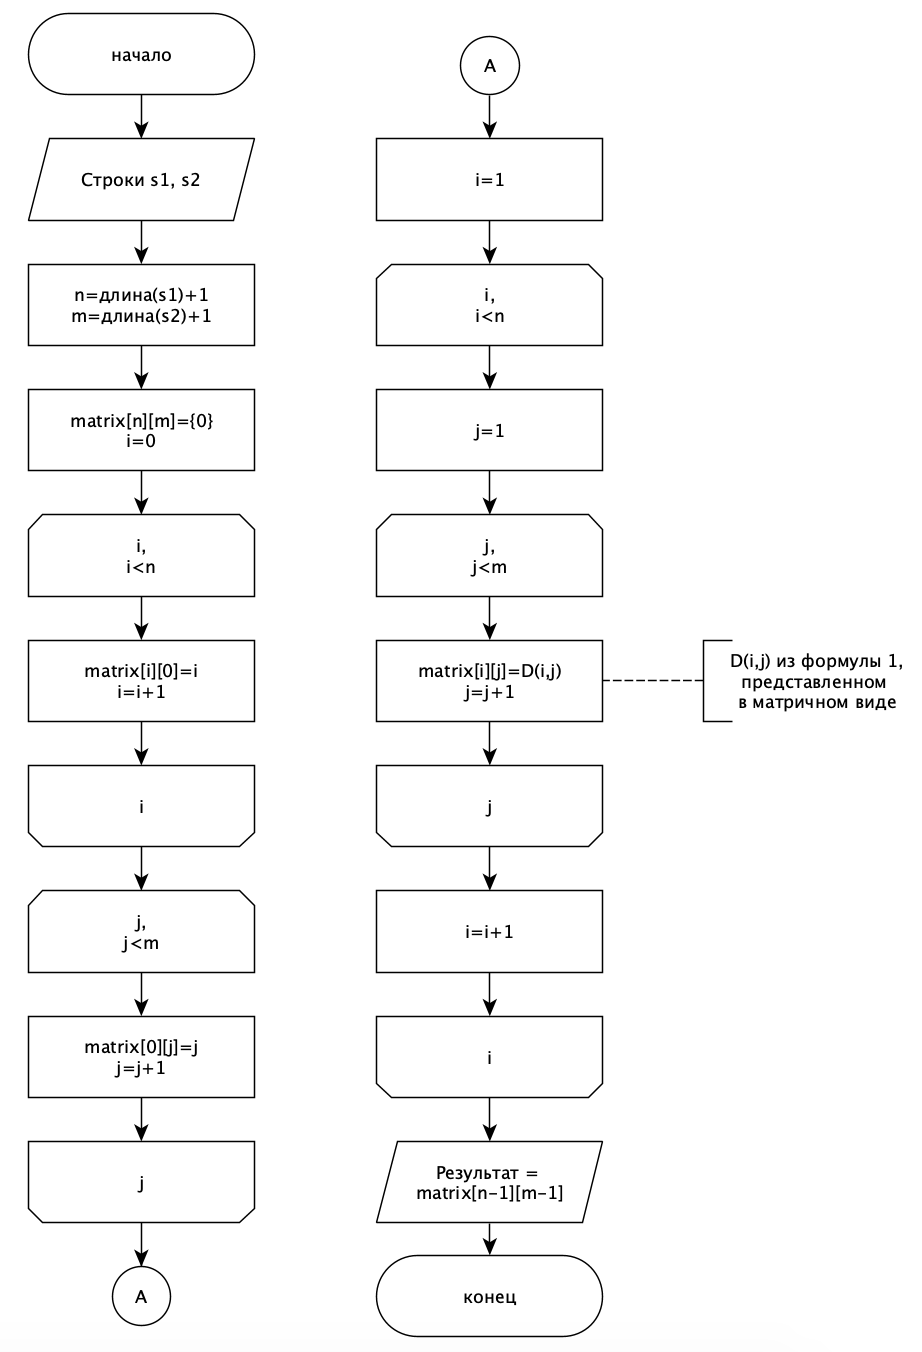
\includegraphics[scale = 0.5]{shema1} \\ Схема  1 - алгоритм нахождения расстояния Левенштейна матричным способом
	\end{center}
	
        \subsubsection{Расстояние Дамерау-Левенштейна матричным способом}
        
        \begin{center}
        		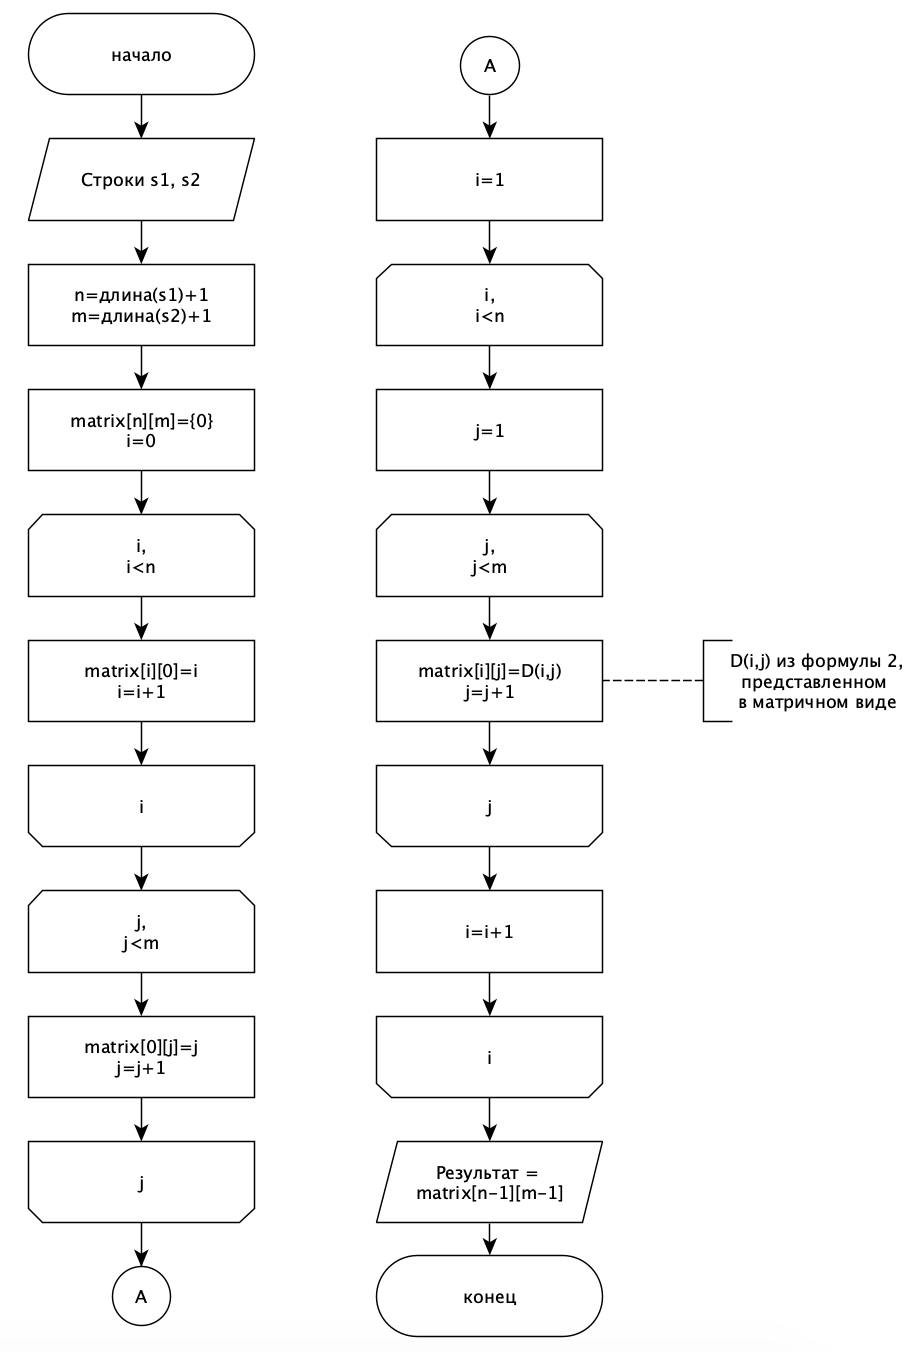
\includegraphics[scale = 0.5]{shema2} \\ Схема  2 - алгоритм нахождения расстояния Дамерау-Левенштейна матричным способом
	\end{center}
	
	\subsubsection{Расстояние Дамерау-Левенштейна рекурсивным способом}
	
	\begin{center}
        		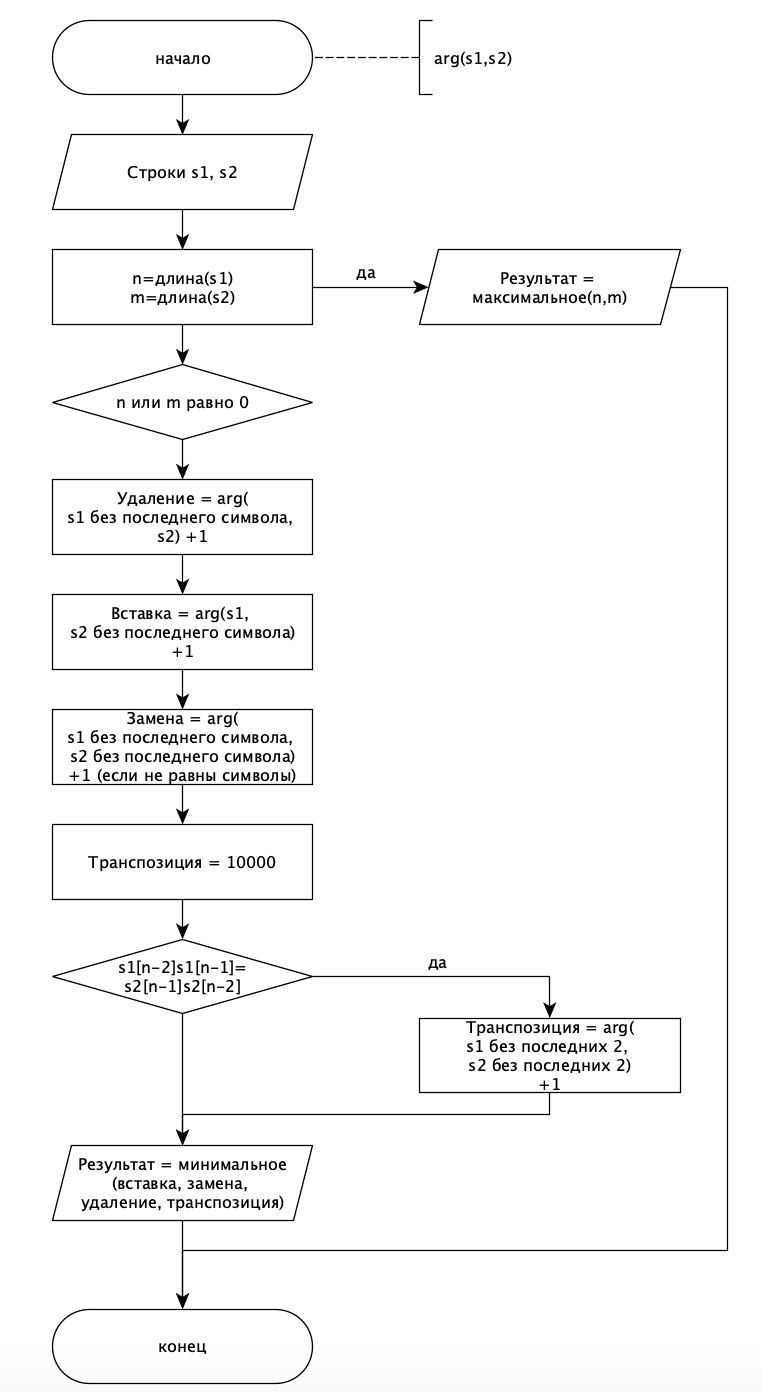
\includegraphics[scale = 0.5]{shema3} \\ Схема  3 - алгоритм нахождения расстояния Дамерау-Левенштейна рекурсивным способом
	\end{center}	
	
	\subsection{Выводы}
	\hfill
	
	В самом коротком пути рекурсивный алгоритм нахождения расстояния Дамерау-Левенштейна имеет сложность $\Omega(4^{min(m,n)})$, а в максимальная длина $\Omega(4^{m + n + 1})$, матричная реализация имеет сложность $\Omega(mn)$. Следует вывод, что рекурсивная реализация является гораздо более затратной по времени. Реализуем алгоритмы поиска редакторских расстояний и проверим наше предположение. 

    \newpage

        \section{Технологическая часть}
        
        \hfill
        
        Стоит задача разработки и сравнительного анализа алгоритмов, вычисляющих редакторские расстояния. 
        \hfill
        
        В реализациях в целях увеличения точности подсчета времени вывод матрицы был вынесен за пределы функций-алгоритмов. В целях наглядности были опущены части программ, не относящиеся к работе алгоритмов.
        
        \subsection{Требования к программному обеспечению}
        \hfill
        
        ПО должно предоставлять возможность замеров процессорного времени выполнения реализации каждого алгоритма. Требуется провести замеры для варьирующихся длин строк: от 100 до 1000. Один эксперимент ставится не менее 100 раз, результат одного эксперимента рассчитывается как среднее значение результатов проведенных испытаний с одинаковыми входными данными.
        \hfill
        
        Используемое ПО - Mac OS. 
        \subsection{Средства реализации}
        \hfill
        
        В качестве языка программирования был выбран Python. 
        \hfill
        
        Python -- высокоуровневый язык программирования общего назначения, ориентированный на повышение производительности разработчика и читаемости кода. Синтаксис Python минималистичен. В то же время стандартная библиотека включает большой объём полезных функций.
        \hfill
        
        Python обладает динамической типизацией, автоматическим управлением памятью.
        
        \subsection{Листинг кода}
        \textbf{Расстояние Левинштейна, матричный способ: }
        
	\begin{lstlisting}
	def levinstein(s1, s2):
 	    n_matrix = len(s1) + 1
 	    m_matrix = len(s2) + 1
 	    matrix = [[0] * m_matrix for i in range(n_matrix)]

 	    for i in range(n_matrix):
  	 	matrix[i][0] = i
 	    for j in range(m_matrix):
 		matrix[0][j] = j

 	    for i in range(1, n_matrix):
   		for j in range(1, m_matrix):
   		    matrix[i][j] = min(matrix[i - 1][j] + 1, matrix[i][j - 1] + 1,
   	   	    matrix[i - 1][j - 1] + (s1[i - 1] != s2[j - 1]))
 
 	    return matrix[n_matrix - 1][m_matrix - 1]
	\end{lstlisting}

	\textbf{Расстояние Дамерау-Левинштейна, матричный способ: }
	\begin{lstlisting}
	def damerau_levinstein_matrix(s1, s2):
	    n_matrix = len(s1) + 1
	    m_matrix = len(s2) + 1
   	    matrix = [[0] * m_matrix for i in range(n_matrix)]

 	    for i in range(n_matrix):
  	        matrix[i][0] = i
 	    for j in range(m_matrix):
  	        matrix[0][j] = j

 	    for i in range(1, n_matrix):
   		for j in range(1, m_matrix):
    	             if (i > 1 and s1[i - 1] == s2[j - 2] and s1[i - 2] == s2[j - 1]):
     	                 matrix[i][j] = min(matrix[i - 1][j] + 1, 
	                 matrix[i][j - 1] + 1, matrix[i - 1][j - 1] + 
	                 (s1[i - 1] != s2[j - 1]), matrix[i - 2][j - 2] + 1)
   	             else:
   	                 matrix[i][j] = min(matrix[i - 1][j] + 1, 
	                 matrix[i][j - 1] + 1, matrix[i - 1][j - 1] + 
	                 (s1[i - 1] != s2[j - 1]))

 	    return matrix[n_matrix - 1][m_matrix - 1]
	\end{lstlisting}

	\textbf{Расстояние Дамерау-Левинштейна, рекурсивный способ: }
	\begin{lstlisting}
	def damerau_levinstein_recursive(s1, s2):
	    n = len(s1)
	    m = len(s2)
	    if (0 == n):
  	        return m
	    if (0 == m):
  	        return n

	    delete = damerau_levinstein_recursive(s1[:-1], s2) + 1
	    insert = damerau_levinstein_recursive(s1, s2[:-1]) + 1
	    replace = damerau_levinstein_recursive(s1[:-1], s2[:-1]) + 
	    (s1[-1] != s2[-1])
	    transposition = 1000
	    if (n > 1 and m > 1 and s1[-1] == s2[-2] and s1[-2] == s2[-1]):
  	        transposition = damerau_levinstein_recursive(s1[:-2], s2[:-2]) + 1

	    return min(delete, insert, replace, transposition)
	\end{lstlisting}

	\subsection{Тестирование}
	\hfill
	
	В таблице 1 представлена заготовка данных для тестирования наших алгоритмов. 
	\begin{center}
		\begin{tabular}{ | l | l | l |}
			\hline
			\textbf{Строка1} & \textbf{Строка2} & \textbf{Ожидаемый результат} \\ \hline
			dessert & desert & 1 \\ \hline
			cook & cooker & 2 \\ \hline
			mother & money & 3 \\ \hline
			woman & water & 4 \\ \hline
			program & friend & 6 \\ \hline
			house & girl & 5 \\ \hline
			probelm & problem & 1 or 2 \\ \hline
			head & ehda & 2 or 3 \\ \hline
			bring & brought & 4 \\ \hline
			happy & happy & 0\\  \hline
			minute & moment & 5 \\ \hline
			person & eye & 5 \\ \hline
			week & weeks & 1 \\ \hline
			member & morning & 6 \\ \hline
			death & health & 2 \\ \hline
			education & question & 4 \\ \hline
			room & moor & 2 \\ \hline
			car & city & 3 \\ \hline
			air & area & 3 \\ \hline
			country & office & 6 \\ \hline
		\end{tabular}
		
		\hfill
		
		Таблица 1.
		Подготовленные тестовые данные.  
	\end{center}
	\subsection{Выводы}
	
        \hfill
        
        Реализовано 3 алгоритма, подготовлены тесты для оценки качества их работы. 
        
        Получены практические навыки реализации матричного поиска расстояния Левинштейна и матричного и рекрсивного -- Дамерау-Левенштейна. 

    \newpage

        \section{Экспериментальная часть}
        \hfill
        
        Оценка качества работы алгоритмов. Экспериментальное сравнение работы различных алгоритмов (зависимость времени выполнения от длины входных слов). 
        
        \subsection{Примеры работы}
	\hfill
	
	На рисунке 2 представлены примеры работы программы на разных входных данных. 
	\begin{figure}[ht]\center
		\begin{tabular}{cc}
			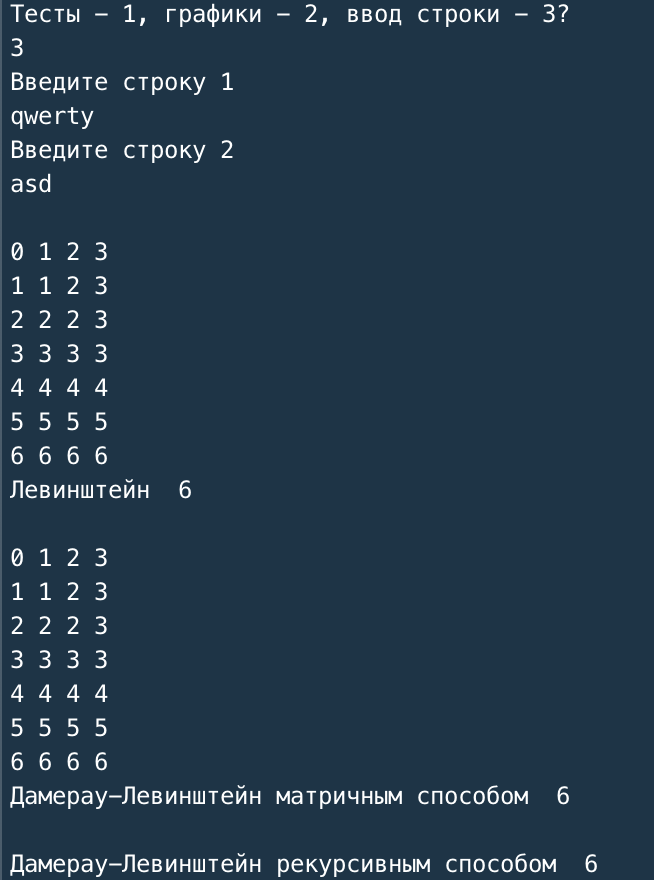
\includegraphics[width=50mm]{ex1} & 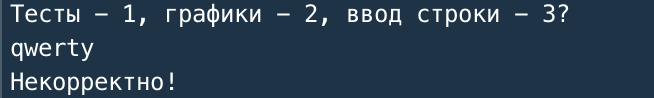
\includegraphics[width=50mm]{ex2} & 
			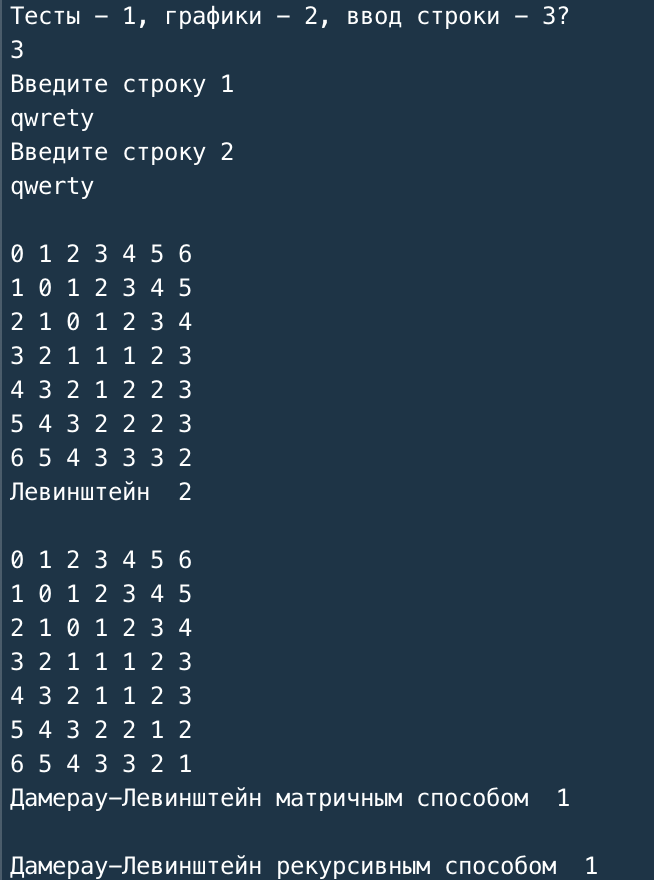
\includegraphics[width=50mm]{ex3} & 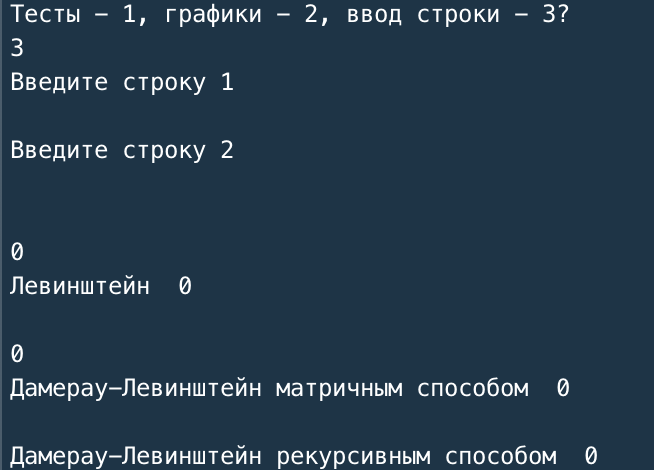
\includegraphics[width=50mm]{ex4}
		\end{tabular}
		\\ Рис. 2 - Примеры работы
	\end{figure}
        
        \subsection{Результаты тестирования}
        
	\hfill
	
	Проверяем нашу программу на тестах из таблицы 1. Полученные результаты представлены в таблице 2. 
	
	\begin{center}
       		\begin{tabular}{ | l | l | l | l | l |}
			\hline
			\textbf{Строка1} & \textbf{Строка2} & \textbf{Л. матричный} & \textbf{Д.-Л. матричный}  & \textbf{Д.-Л. рекурсивный}\\ \hline
			dessert  &  desert  &  1  &  1  &  1 \\ \hline
			cook  &  cooker  &  2  &  2  &  2 \\ \hline
			mother  &  money  &  3  &  3  &  3 \\ \hline
			woman  &  water  &  4  &  4  &  4 \\ \hline
			program  &  friend  &  6  &  6  &  6 \\ \hline
			house  &  girl  &  5  &  5  &  5 \\ \hline
			probelm  &  problem  &  2  &  1  &  1 \\ \hline
			head  &  ehda  &  3  &  2  &  2 \\ \hline
			bring  &  brought  &  4  &  4  &  4 \\ \hline
			happy  &  happy  &  0  &  0  &  0 \\ \hline
			minute  &  moment  &  5  &  5  &  5 \\ \hline
			person  &  eye  &  5  &  5  &  5 \\ \hline
			week  &  weeks  &  1  &  1  &  1 \\ \hline
			member  &  morning  &  6  &  6  &  6 \\ \hline
			death  &  health  &  2  &  2  &  2 \\ \hline
			education  &  question  &  4  &  4  &  4 \\ \hline
			room  &  moor  &  2  &  2  &  2 \\ \hline
			car  &  city  &  3  &  3  &  3 \\ \hline
			air  &  area  &  3  &  3  &  3 \\ \hline
			country  &  office  &  6  &  6  &  6 \\ \hline
		\end{tabular}
		
		\hfill
		
		Таблица 2.
		Тестирование программы.  
	\end{center}
	
	\hfill
	
	\textbf{Тесты пройдены}

	\subsection{Замеры времени}
	
	\hfill
	
	На графиках 1-3 представлено сравнение алгоритмов поиска редакционного расстояния по времени. 
	
	\begin{center}
        		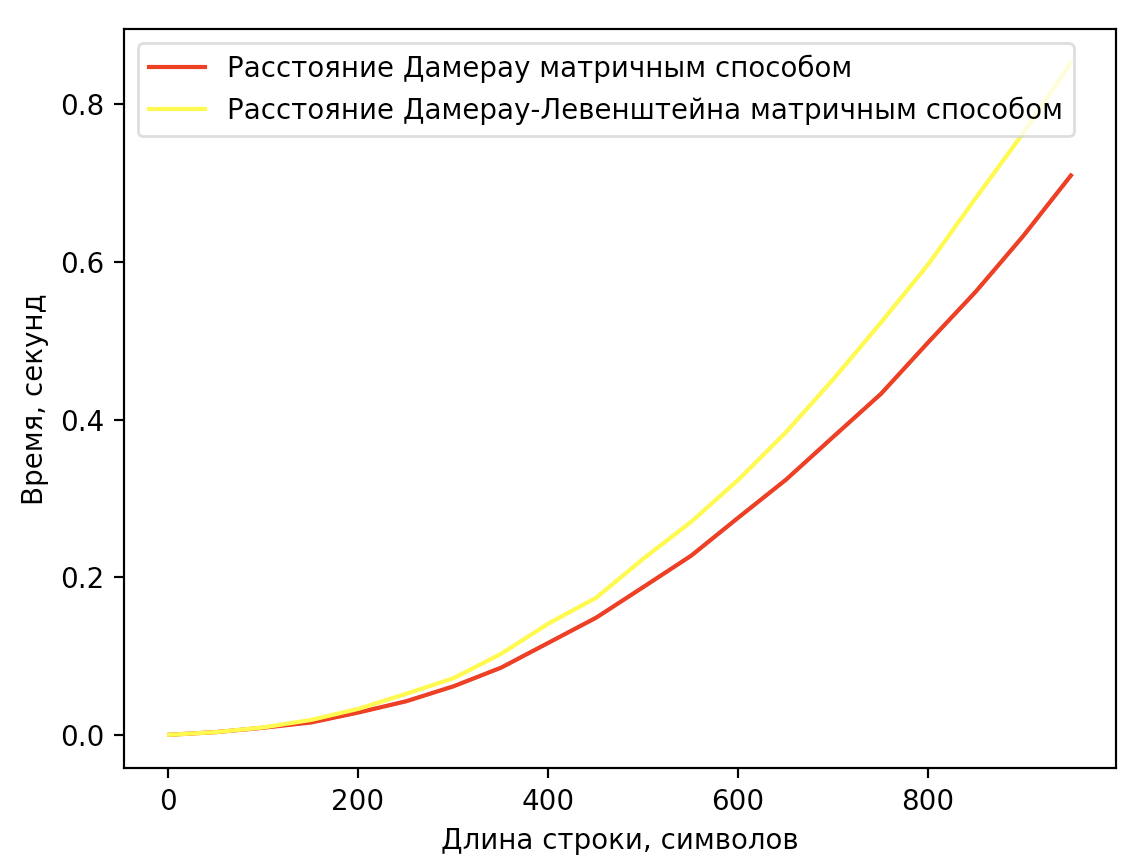
\includegraphics[scale = 0.5]{graph1} \\ График 1 - Сравнение реализации алгоритмов нахождения расстояний Левенштейна и Дамерау-Левенштейна матричным способом
	\end{center}
	
	\begin{center}
        		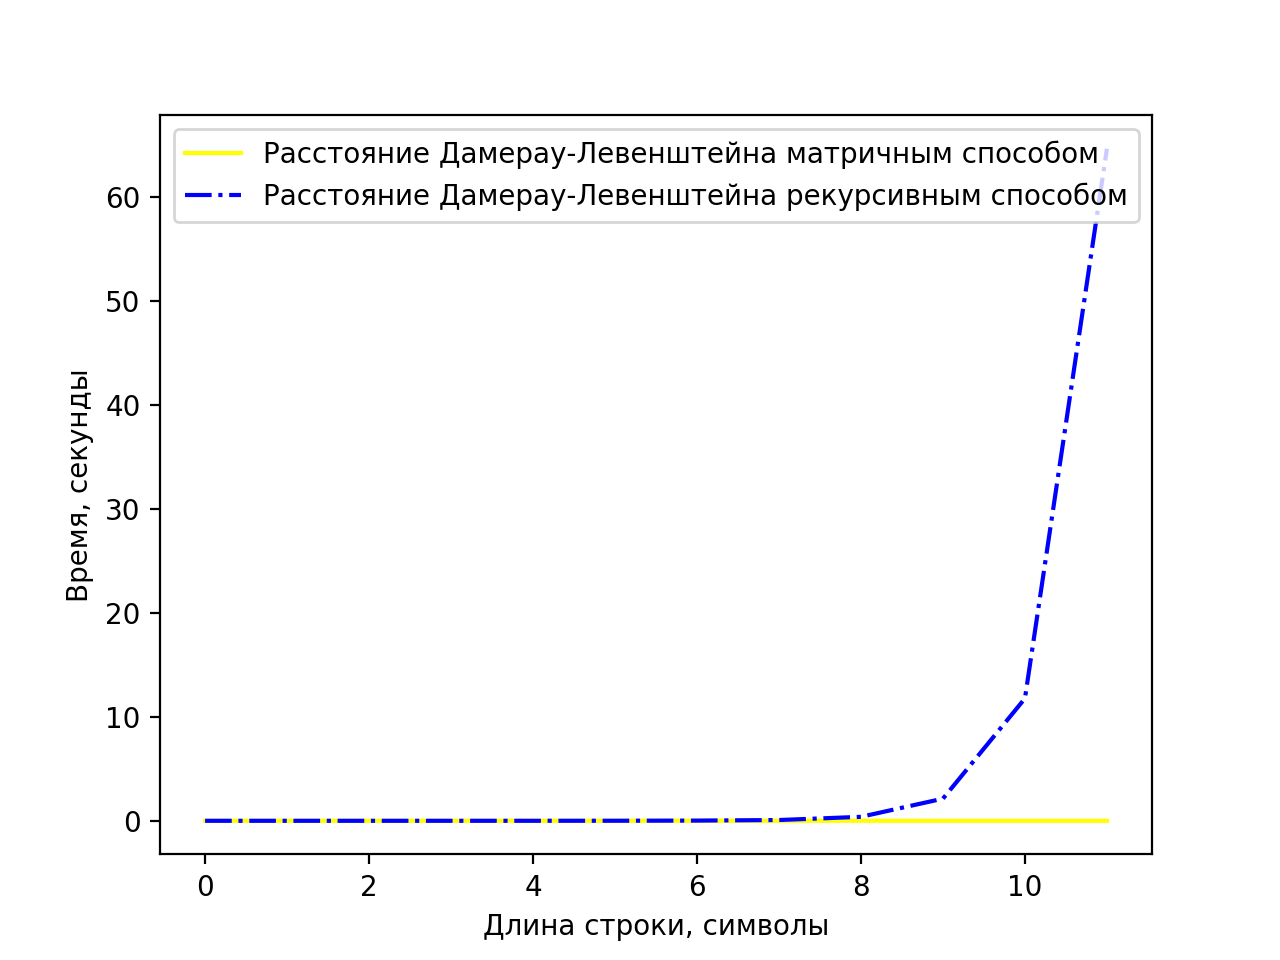
\includegraphics[scale = 0.5]{graph2} \\ График 2 - Сравнение реализации алгоритмов нахождения расстояния Дамерау-Левенштейна матричным и рекурсивным способом
	\end{center}
	
	\begin{center}
        		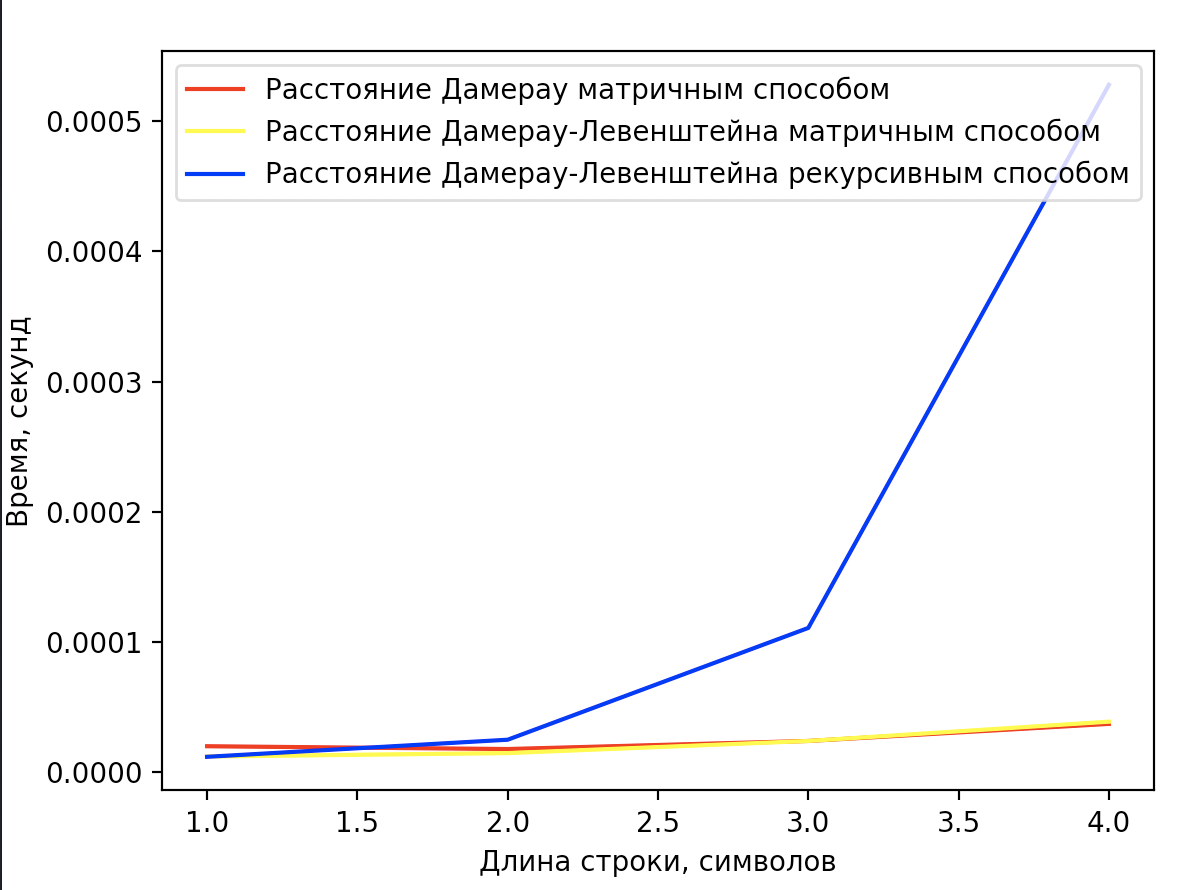
\includegraphics[scale = 0.5]{graph3} \\ График 3 - Сравнение реализации всех 3 алгоритмов
	\end{center}
	
	\subsection{Выводы}
	\hfill
	
	Как видно из графиков рекурсивный алгоритм является самым медленным, гораздо быстрее использовать алгоритмы матричные. Дамерау-Левенштейна проигрывает обычному Левенштейну только на очень больших длинах слов, но цена ошибки, в некоторых случаях, у него меньше.
   	\newpage

        \anonsection{Заключение}
        
        \hfill
        
	В данной лабораторной работе было реализовано и пронализировано 3 алгоритма нахождения редакционных расстояний:
	\begin{enumerate}
	 	\item нахождение расстояния Левенштейна матричным способом \\
		\item нахождение расстояния Дамерау-Левенштейна матричным способом \\
		\item нахождение расстояния Дамерау-Левенштейна рекурсивным способом \\
	\end{enumerate}
	
	Расстояние Левенштейна и его модификация активно применяются:
	\begin{enumerate}
		\item для исправления ошибок в слове (компьютерная или машинная лингвистика)
		\item для сравнения текстовых файлов утилитой diff и ей подобными
		\item в биоинформатике для сравнения генов, хромосом и белков
	\end{enumerate}
	
	\hfill
	
	При сравнении данных алгоритмов пришли к следующим выводам:
	\begin{enumerate}
 		\item Рекурсивный алгоритм является самым медленным, гораздо быстрее использовать алгоритмы матричные.   \\
 		\item Дамерау-Левенштейна проигрывает обычному Левенштейну только на очень больших длинах слов, но цена ошибки, в некоторых случаях, у него меньше.\\
	\end{enumerate}

 	\newpage

        \begin{thebibliography}{3}
		\bibitem{} Сложность дистанции редактирования (расстояние Левенштейна)[Электронный ресурс]. -- Режим доступа: http://qaru.site/questions/3908099/complexity-of-edit-distance-levenshtein-distance-recursion-top-down-implementation (дата обращения: 15.09.2019).
		\bibitem{} Вычисление редакционного расстояния[Электронный ресурс]. -- Режим доступа: https://habr.com/ru/post/117063/ (дата обращения: 15.09.2019).
		\bibitem{} Нечёткий поиск в тексте и словаре[Электронный ресурс]. -- Режим доступа: https://habr.com/ru/post/114997/ (дата обращения: 15.09.2019).
	\end{thebibliography}

\end{document}
